\section{Final evaluation and results}
\subsection{Evaluation Metrics}
The goal of the evaluation methods was to asses the potential use of the web visualiser. Evaluating user experience was the best way to understand how the visualiser served the purpose users expected it to. Feedback and suggestion given by users were taken and used to improve the effectiveness and accuracy of the visualizer\cite{lam:hal-00723057}

\subsubsection{Effectiveness and Accuracy}
In user interface, effectiveness is used to describe the functionality of a tool and  also evaluates a user's performance when performing tasks. Accuracy on the other hand refers to the way in which data/information is presented to the user. To ensure effectiveness, a lot of affordances and feedback mechanism were employed.
\subsubsection{Usability}
Usability can be described as the measure of  the quality of use of a platform/application by a potential user. This makes it an essential component of visualisation to take into account\cite{1509067}.
\paragraph{}
During usability tests, users were allowed to perform prescribed tasks while their interaction with the interface were observed, their reaction to certain tasks were also taken into account. This was done so that user task completion and tasks success rate could be measured. The main tasks to be performed were chosen based on major features.


\subsection{Usability Tests}
In order to test the effectiveness, accuracy and usability of the visualisation, usability tests were done with eight potential users. Four of these users researchers from UCT while the other four were members of the Ocean View community. 
\paragraph{}
Task completion was used to measure accuracy and effectiveness during the tests while ease of use(ability to navigate the app with ease) was used to gauge usability. A questionnaire consisting of both scales and free response questions were used to collect user feedback.
\paragraph{}
To conduct usability studies, an ethical clearance was obtained from the Department of Student Affairs and the Science Faculty Research Ethics Committee. At the beginning of the usability test, participants were asked to sign a consent form outlining the agreement between the researchers and them. The form also guaranteed them anonymity of their results.
\paragraph{}
The usability study with community member was done first. Participants did the tests individually, one at a time. After performing their tasks and providing feedback,the next user was given their set of tasks to complete which were different from the previous one. The same process was followed with researchers from UCT but with a different set of tasks that were specific to users with working knowledge of computer networks.
\subsection{Analysis of Results}
\subsubsection{Task Completion}
The success of a takes was defined by the attained of different objectives for each task. For some other tasks it can generally be referred to the participant's ability to obtain some data during execution of a certain task. Since participants we observed while performing the task, a participant was said to be successful if they completed the task at hand.
\paragraph{}
From the results, it was observed all users were able to complete certain tasks while others struggled with more involved tasks. The results of the  two sets of tasks are shown on Figure 6 and Figure 7.

\begin{figure}
	\centering
	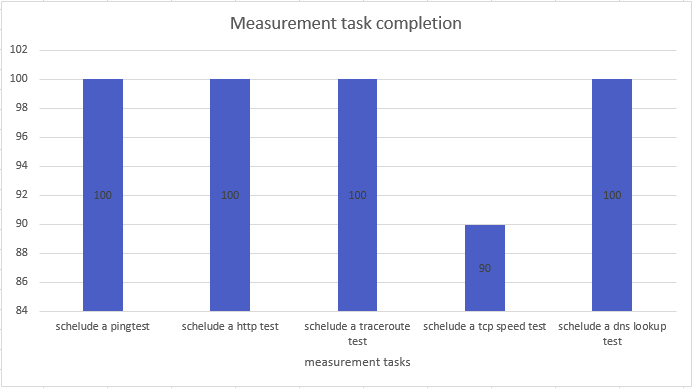
\includegraphics[width=1\linewidth]{images/tasks1}
	\caption{Completion rate of the first set of tasks}
	\label{fig:proto}
\end{figure}

\begin{figure}
	\centering
	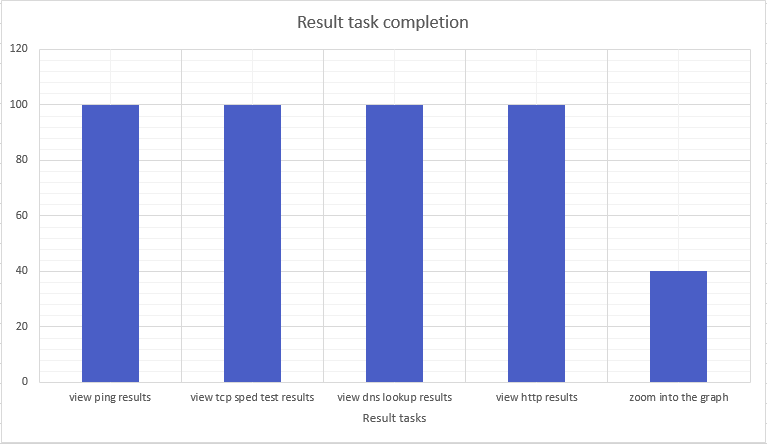
\includegraphics[width=1\linewidth]{images/task2}
	\caption{Completion rate of the second set of tasks}
	\label{fig:proto}
\end{figure}
\subsubsection{User Feedback}
A questionnaire that consisted of a scale and free response questions was given to participants  at the end of each usability test. The free response questions for researchers added were "Do you think the app provides enough information for networking researchers/network administrators?. If not what else would a user want?" and "Do you have any other feedback on the application?". This allowed users to elaborate on their experience with the application.
\paragraph{}
For the Ocean View community members, these were the free response questions "Do you think the app provides enough information for Inethi network users?. If not what else would a user of the network want?" and "What did you like the most about the app for you?".
\paragraph{}
These questions were not compulsory for participants but a significant number of them answered nonetheless. 